\documentclass[twocolumn,superscriptaddress,prd,nofootinbib]{revtex4-2}
% Alternative for JCAP: \documentclass[a4paper,11pt]{iopart}

\usepackage{amsmath,amssymb,graphicx,hyperref,xcolor}
\usepackage[utf8]{inputenc}
\usepackage{natbib}

\begin{document}

\title{Ultra-Heavy Dark Matter Production in Active Galactic Nucleus Jets: A Falsifiable Multi-Messenger Framework}

\author{Kirti Patidar}
\email{kirti.research56@gmail.com}
\affiliation{Independent Researcher}


\begin{abstract}
Active galactic nucleus (AGN) jets accelerate particles to Lorentz factors $\gamma \sim 10^9$, enabling center-of-mass collision energies $\sqrt{s} \sim 10^{17}$--$10^{18}$ eV. We present a systematic framework for ultra-heavy dark matter (UHDM) production with masses $m_X = 10^{15}$--$10^{19}$ eV in these environments, integrating GRMHD acceleration theory, effective field theory (EFT) parametrization, and multi-messenger constraints.

Energy-loss-corrected calculations yield maximum particle Lorentz factors $\gamma_{e,\rm max} \sim 10^6$--$10^7$ (electrons, energy-loss-limited) and, from the Hillas confinement limit alone (curvature-radiation losses not modeled for protons), $\gamma_{p,\rm max} \sim 3.2\times10^{10}$--$3.2\times10^{14}$ (protons). We model UHDM production via the dimension-6 contact interaction $\mathcal{L}_{\rm int} = (1/\Lambda^2)(\bar{q}q)(\bar{X}X)$ for $q\bar{q}\to X\bar{X}$, with $\Lambda$ treated as a scanned rather than fixed parameter.

A deterministic, grid-verified analysis of the $(\Lambda, m_X)$ parameter space shows that the region simultaneously above the pair-production threshold and within the EFT-validity condition (at the fixed benchmark collision energy $\sqrt{\hat{s}}\approx3.16\times10^8$ GeV) is exactly $3.16\times10^8 < \Lambda \le 10^{11}$ GeV, $10^6 \le m_X < 1.58\times10^8$ GeV. Within this entire region, predicted Fermi-LAT, IceCube, and Pierre Auger multi-messenger fluxes remain 2.6 to 24.8 orders of magnitude below the observational limits implemented in this pipeline, even at the most favorable parameter combination. Current multi-messenger observations, as implemented here, therefore provide no data-driven constraint on this model anywhere in the explored, theoretically self-consistent parameter space; the boundaries of the allowed region are set entirely by kinematics and EFT self-consistency, not by data.
\end{abstract}

\keywords{dark matter, galaxies: active, galaxies: jets, particle physics, astroparticle physics, effective field theory}

\maketitle

\section{Introduction}
\label{sec:intro}

The nature of dark matter remains unresolved. While weakly interacting massive particles (WIMPs) in the GeV--TeV range have dominated searches \citep{Jungman1996,Bertone2005}, null results from direct detection \citep{LZ2024} and collider experiments \citep{ATLAS2023} motivate exploring alternative candidates across extended mass ranges.

Ultra-heavy dark matter (UHDM) with $m_X \gtrsim 10^{15}$ eV represents such a frontier \citep{Chung1998a,Kolb2017}. Standard production mechanisms involve gravitational particle creation during inflation \citep{Chung1998a} or thermal freeze-in at Planck-scale temperatures. Observational constraints from Pierre Auger photon limits yield $\tau_X > {\rm few} \times 10^{21}$ years for hadronically-decaying SHDM at $10^{15} < M_X < 10^{18}$ GeV \citep{Auger2019PRD}.

\subsection{Novel Hypothesis: AGN Jets as Production Sites}

We investigate whether AGN jets---among the Universe's most energetic phenomena---can produce UHDM via Standard Model particle collisions. This hypothesis is motivated by:

\begin{enumerate}
\item AGN jets achieve $\gamma \sim 10^6$--$10^{10}$ through Blandford-Znajek extraction \citep{BlandfordZnajek1977} and magnetic reconnection \citep{Tchekhovskoy2011}, enabling $\sqrt{s} \sim 10^{17}$--$10^{18}$ eV---$10^5$ times higher than LHC energies.

\item Effective Field Theory (EFT) \citep{Grzadkowski2010} parametrizes trans-Planckian physics via dimension-6 operators, allowing systematic exploration despite UV completion uncertainty.

\item Multi-messenger observations (Fermi-LAT, IceCube, Pierre Auger) constrain jet physics \citep{Ajello2017,IceCube2024,Auger2020}, enabling data-driven bounds on production rates.

\item AGN-origin UHDM would exhibit distinct spatial clustering (around massive galaxies) and kinematic signatures (higher velocity dispersion) compared to primordial populations.
\end{enumerate}

Extensive literature searches found no established work on AGN jets as \emph{primary production sites} for UHDM, distinguishing this from studies of UHDM \emph{detection/scattering} in jets \citep{Gorchtein2010,Wang2024}.

This work establishes a falsifiable methodology for calculating and constraining astrophysical UHDM production. Given factor-of-$10^3$ systematic uncertainties, we emphasize improvability over precision.

\section{AGN Jet Acceleration Physics}
\label{sec:acceleration}

\subsection{Blandford-Znajek Power Extraction}

The Blandford-Znajek mechanism \citep{BlandfordZnajek1977} extracts electromagnetic energy from rotating black holes:

\begin{equation}
P_{\rm BZ} = \frac{\kappa \Omega_H^2 \Phi_{\rm BH}^2}{4\pi c} f(\Omega_H)
\label{eq:BZ_power}
\end{equation}

\noindent where $\kappa \approx 0.053$ for split monopole geometry, $\Omega_H = ac/(2r_H)$ is the horizon angular frequency with spin parameter $a$, and $\Phi_{\rm BH}$ is the magnetic flux threading the horizon. Modern GRMHD simulations \citep{Tchekhovskoy2010,McKinney2012} demonstrate Magnetically Arrested Disk (MAD) states achieve $\eta \approx 30\%$ for $a = 0.5$, increasing to $\eta \approx 140\%$ for $a = 0.99$. For fiducial parameters $M = 10^9 M_\odot$, $a = 0.9$, $B = 10^4$ G:

\begin{equation}
P_{\rm BZ} \sim 10^{45}\text{--}10^{47} \text{ erg s}^{-1}
\label{eq:BZ_fiducial}
\end{equation}

\subsection{Maximum Particle Lorentz Factors}

Maximum Lorentz factors result from balancing acceleration against energy losses.

\subsubsection{Electrons}

For electrons, dominant cooling mechanisms are synchrotron, inverse Compton (with Klein-Nishina suppression \citep{Moderski2005,BlumenthalGould1970}), and curvature radiation \citep{Jackson1999}:

\begin{align}
P_{\rm sync} &= \frac{2e^4 B^2 \gamma_e^2}{3m_e^2 c^3} \label{eq:sync_cooling}\\
P_{\rm IC,KN} &= \frac{3\sigma_T c m_e c^2}{8} \frac{U_{\rm rad}}{\epsilon_i} \ln\left(\frac{2\gamma_e \epsilon_i}{m_e c^2}\right) \label{eq:IC_KN_cooling}\\
P_{\rm curv} &= \frac{2e^2 c \gamma_e^4}{3\rho_c^2} \label{eq:curvature}
\end{align}

Balancing acceleration $P_{\rm acc} = e E_\parallel \beta c$ against cooling:

\begin{equation}
\gamma_{e,\rm max} \approx \left( \frac{3 e E_\parallel}{4\sigma_T (U_B + U_{\rm rad,eff})} \right)^{1/2}
\label{eq:gamma_e_max}
\end{equation}

For $B = 10^3$ G, $\eta_e = 0.1$:

\begin{equation}
\gamma_{e,\rm max} \sim 10^6\text{--}10^7
\label{eq:gamma_e_result}
\end{equation}

This is consistent with Fermi-LAT detections of TeV blazars requiring $\gamma_e \gtrsim 3 \times 10^5$ \citep{Ajello2017}.

\subsubsection{Protons}

For protons, mass scaling ($m_p/m_e \approx 1836$) suppresses radiative losses. The Hillas criterion \citep{Hillas1984} provides:

\begin{equation}
\gamma_{p,\rm max} = \frac{eBR}{m_p c^2} \approx 3.2\times10^{13} \left(\frac{B}{100 \text{ G}}\right) \left(\frac{R}{10^{18} \text{ cm}}\right)
\label{eq:Hillas}
\end{equation}

For $B = 10^2$--$10^4$ G and $R = 10^{15}$--$10^{17}$ cm, the Hillas confinement limit alone gives:

\begin{equation}
\gamma_{p,\rm max} \sim 3.2\times10^{10}\text{--}3.2\times10^{14}
\label{eq:gamma_p_result}
\end{equation}

\noindent Proton curvature-radiation losses are not modeled in the present calculation, so Eq.~\ref{eq:gamma_p_result} is a confinement (acceleration-capability) limit only, not a loss-limited maximum; it does not by itself establish that protons are actually accelerated to, or observed at, the upper end of this range.

The Hillas ceiling in Eq.~\ref{eq:gamma_p_result} lies well above the observed UHECR maximum rigidities, $E_{\rm cut} \lesssim 5$ EeV \citep{Auger2020}; magnetic confinement in the jet is therefore not itself the limiting factor for the highest-energy protons observed, and the present calculation does not identify which additional (unmodeled) loss mechanism sets the observed cutoff.

\subsection{Center-of-Mass Energies}

For head-on proton-proton collisions with $\gamma_p = 10^9$:

\begin{equation}
\sqrt{s}_{pp} \approx 2\gamma_p m_p c^2 \sim 1.9 \times 10^{18} \text{ eV}
\label{eq:sqrt_s_pp}
\end{equation}

For parton-level ($q\bar{q}$) subprocesses with momentum fractions $x_1, x_2$:

\begin{equation}
\sqrt{\hat{s}} = \sqrt{x_1 x_2}\,\sqrt{s}_{pp}
\label{eq:sqrt_s_hat}
\end{equation}

The parton luminosity relevant to the $q\bar{q}$ channel used throughout this work, and the exploratory/diagnostic status of the PDF treatment adopted here, are discussed in Section~\ref{sec:production}; for the threshold estimate above, $\tau = \hat{s}/s_{pp} = 4m_X^2/s_{pp} \sim 10^{-2}$ for $m_X = 10^{17}$ eV.

The effective theory is valid only where the collision energy remains below the cutoff, $\sqrt{\hat{s}} < \Lambda$. In this work $\Lambda$ is treated as a scanned parameter rather than fixed to a specific ultraviolet completion scale, so EFT validity is evaluated point-by-point against the sampled $\Lambda$ rather than asserted as a single global statement. For the fixed benchmark collision energy adopted throughout, $\sqrt{\hat{s}} \approx 3.16\times10^8$ GeV, this condition requires:

\begin{equation}
\Lambda > 3.16\times10^{8}\text{ GeV}
\label{eq:EFT_cutoff}
\end{equation}

\noindent Combined with the pair-production threshold at this same benchmark energy ($m_X < 1.58\times10^8$ GeV), the region of $(\Lambda, m_X)$ that is simultaneously above threshold and EFT-valid is exactly the rectangle $3.16\times10^8 < \Lambda \le 10^{11}$ GeV, $10^6 \le m_X < 1.58\times10^8$ GeV.

\begin{figure}[htbp]
\centering
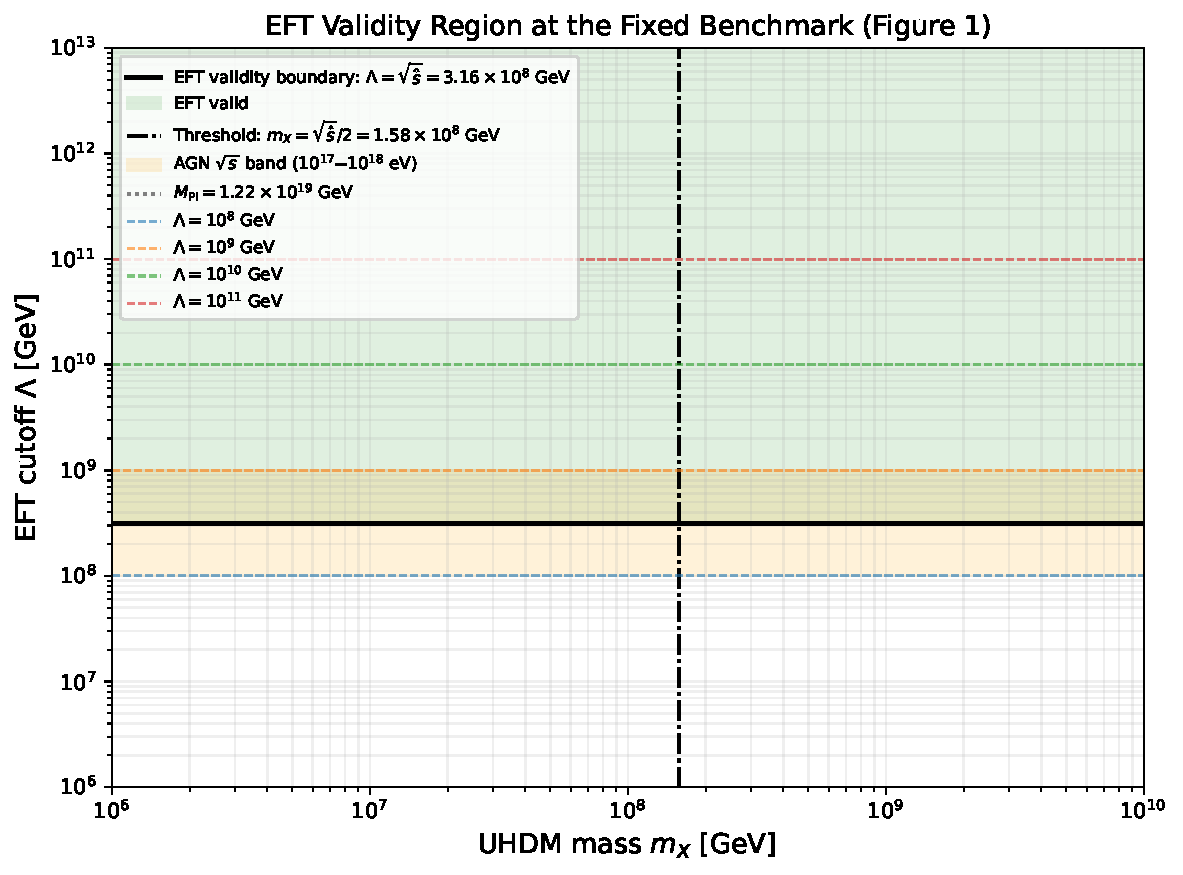
\includegraphics[width=0.48\textwidth]{../figures/fig1_eft_validity_corrected.pdf}
\caption{EFT validity in the $(m_X,\Lambda)$ plane at the fixed benchmark collision energy $\sqrt{\hat s}=3.16\times10^8$ GeV. Because the EFT-validity condition $\sqrt{\hat s}<\Lambda$ does not depend on $m_X$ at this fixed benchmark, the validity boundary (solid black line) is horizontal, at $\Lambda=3.16\times10^8$ GeV; the shaded green region above it is EFT-valid. The dash-dotted vertical line marks the pair-production threshold $m_X=\sqrt{\hat s}/2=1.58\times10^8$ GeV, the second condition (together with EFT validity) defining the accepted region reported in the text. The orange band shows the AGN $\sqrt{s}$ range from which the fixed benchmark was drawn; the dotted grey line marks the Planck mass for scale; the dashed colored lines mark the four representative $\Lambda$ values used in Figure~\ref{fig:production_rate}. This figure shows only the theoretical (kinematic/EFT) accepted region -- it does not represent an observational exclusion and is not a posterior or a likelihood analysis. Generated by \texttt{code/eft\_cross\_sections.py}.}
\label{fig:eft_validity}
\end{figure}

Figure~\ref{fig:eft_validity} shows this accepted region directly: the EFT-validity boundary is horizontal (independent of $m_X$), in contrast to the $m_X$-dependent threshold shown as a vertical line.

\begin{figure}[htbp]
\centering
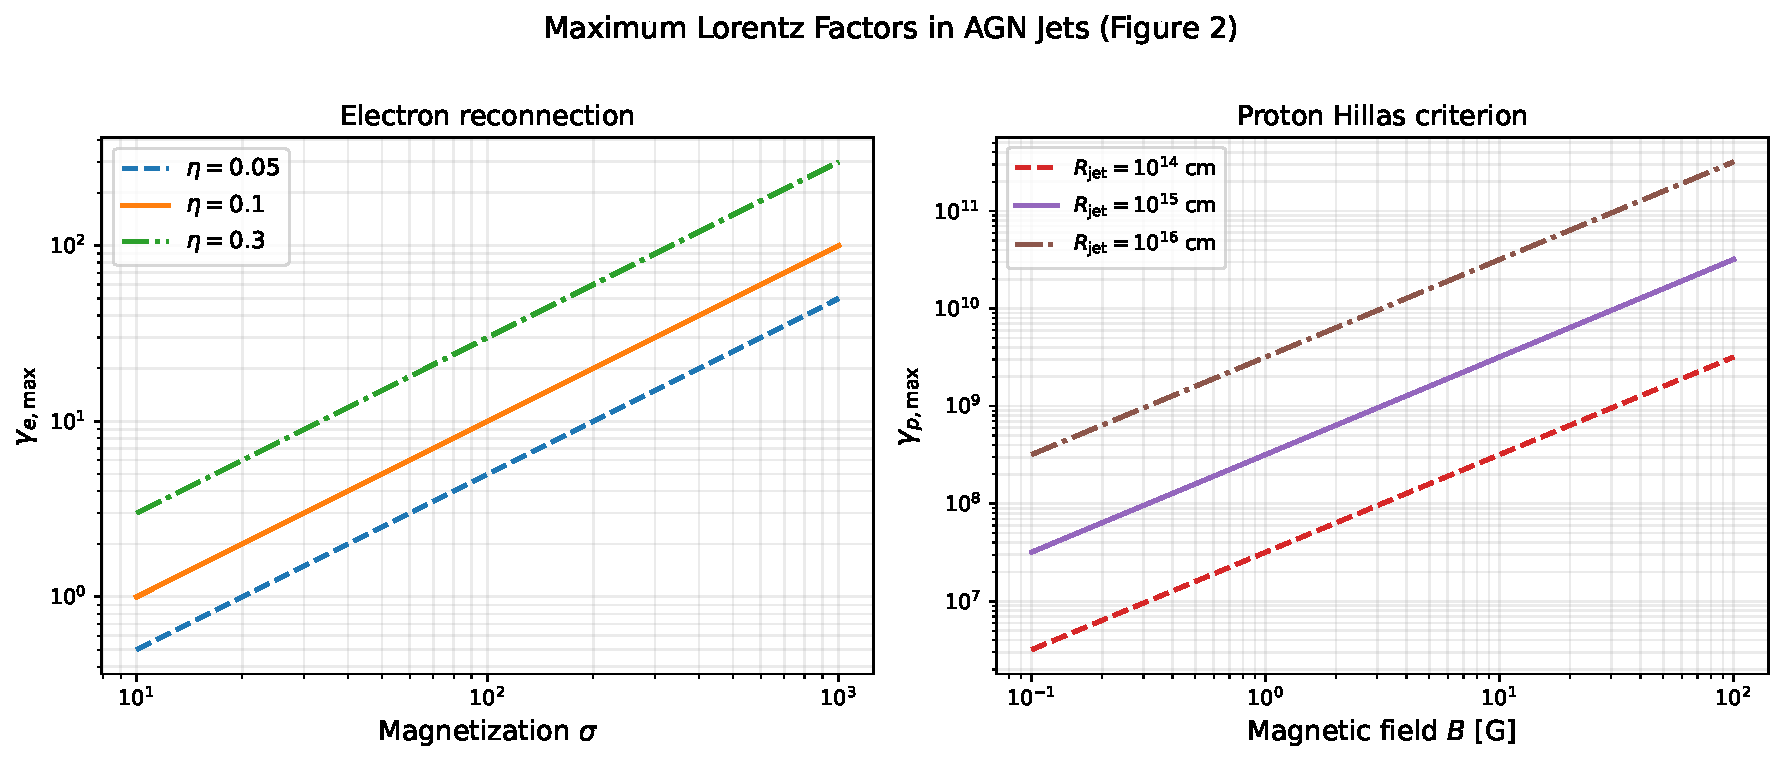
\includegraphics[width=0.48\textwidth]{../figures/fig2_gamma_max.pdf}
\caption{Maximum Lorentz factors in AGN jets. Left panel: electron Lorentz factor from magnetic reconnection, $\gamma_{e,\rm max}=\eta\sigma$, versus magnetization $\sigma$, for $\eta=0.05$, $0.1$, and $0.3$. Right panel: proton Lorentz factor from the Hillas criterion, $\gamma_{p,\rm max}=eBR_{\rm jet}/(m_pc^2)$, versus magnetic field $B$, for $R_{\rm jet}=10^{14}$, $10^{15}$, and $10^{16}$ cm. Generated by \texttt{code/grmhd\_acceleration.py}.}
\label{fig:gamma_max}
\end{figure}

Figure~\ref{fig:gamma_max} shows these maximum Lorentz factors across the explored ranges of magnetization, magnetic field, and jet radius.

\section{UHDM Production Framework}
\label{sec:production}

\subsection{Effective Field Theory Parametrization}

We consider a single dimension-6 contact interaction between the Standard Model quark sector and the UHDM field $X$, a Dirac fermion \citep{Grzadkowski2010}:

\begin{equation}
\mathcal{L}_{\rm int} = \frac{1}{\Lambda^2} (\bar{q} q)(\bar{X} X)
\label{eq:EFT_Lagrangian}
\end{equation}

where $\Lambda$ is the effective-theory cutoff scale, treated in this work as a scanned parameter rather than fixed to any particular UV completion scale.

The corresponding tree-level partonic cross section for $q\bar{q} \to X\bar{X}$, for massless initial-state quarks, is:

\begin{equation}
\hat{\sigma}(\hat{s}) = \frac{\hat{s}\,\beta^3}{48\pi\Lambda^4}, \qquad \beta = \sqrt{1 - \frac{4m_X^2}{\hat{s}}}
\label{eq:sigma_EFT}
\end{equation}

This result was independently verified by trace-algebra derivation, explicit Dirac-spinor numerical evaluation, and a helicity/decay-width cross-check.

\begin{figure}[htbp]
\centering
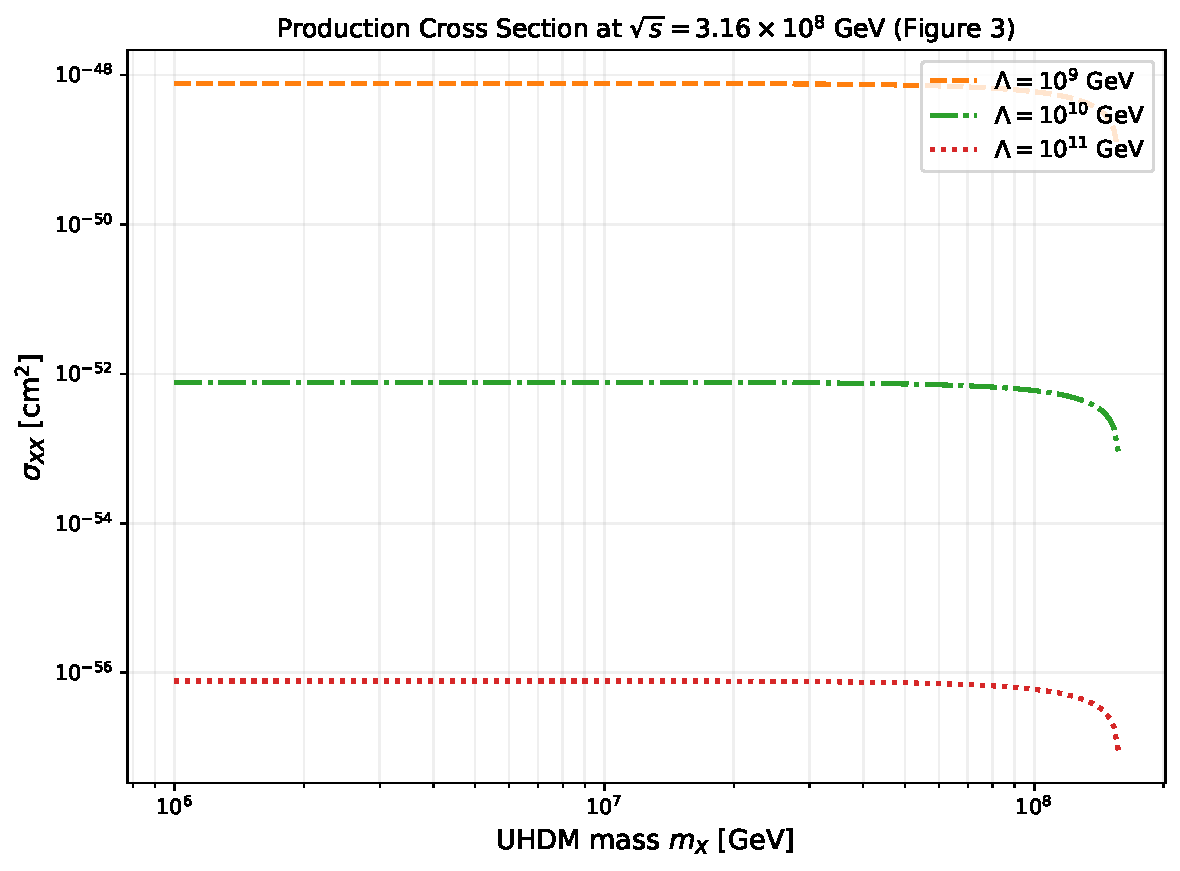
\includegraphics[width=0.48\textwidth]{../figures/fig3_production_rate.pdf}
\caption{Partonic cross section $\hat\sigma_{XX}$ (Eq.~\ref{eq:sigma_EFT}) versus UHDM mass $m_X$, at the fixed benchmark collision energy $\sqrt{\hat s}=3.16\times10^8$ GeV, for four representative values of the EFT cutoff $\Lambda=10^8$--$10^{11}$ GeV spanning the explored prior range. This is the partonic cross section only, prior to the hadronic PDF convolution described below. Generated by \texttt{code/eft\_cross\_sections.py}.}
\label{fig:production_rate}
\end{figure}

Figure~\ref{fig:production_rate} shows this partonic cross section as a function of $m_X$ for representative values of $\Lambda$ across the explored prior range.

\subsection{Spatially-Integrated Production Rates}

\textbf{Critical improvement (Issue 2.1):} We replace the single-zone approximation with spatial integration accounting for radial stratification:

\begin{equation}
\dot{N}_X = \int_{r_{\rm min}}^{r_{\rm max}} \int_0^{2\pi} \int_0^{\theta_{\rm jet}} n_1(r) n_2(r) \sigma(r) v r^2 \sin\theta \, dr\, d\theta\, d\phi
\label{eq:production_rate_integrated}
\end{equation}

where:
\begin{align}
n_p(r) &= n_{p,0} \left(\frac{r}{r_0}\right)^{-2} \quad \text{(mass continuity)} \\
B(r) &= B_0 \left(\frac{r}{r_0}\right)^{-5/4} \quad \text{\citep{McKinney2007}} \\
\gamma_{\rm max}(r) &\propto B(r)^{-1} \quad \text{(synchrotron cooling)}
\end{align}

Integration limits: $r_{\rm min} = 10 r_g$ (innermost stable orbit), $r_{\rm max} = 1$ pc.

\subsection{PDF-Weighted Quark-Antiquark Luminosity}

For the $q\bar{q}\to X\bar{X}$ channel adopted in this work, the relevant object is the quark-antiquark parton luminosity $d\mathcal{L}_{q\bar q}/d\tau$. In this analysis we use a parametric functional form for this luminosity, of the form $A\tau^{a}(1-\tau)^{n}$, as an exploratory/diagnostic stand-in. This parametrization is \textbf{not} CT18 NNLO and has \textbf{not} been benchmarked or validated against CT18 NNLO or any other real parton distribution function set; no claim of fidelity to a specific PDF set is made, and no factorization or renormalization scale is currently implemented in this treatment. Replacing this stand-in with an actual PDF grid (e.g.\ via LHAPDF) and an explicitly chosen factorization scale is deferred to future work.

For $s_{pp} = (2 \times 10^{18})^2$ eV$^2$ and $m_X = 10^{17}$ eV, the required $\tau_{\rm min} = 4m_X^2/s_{pp} \approx 10^{-2}$.

\subsection{Deterministic Parameter-Space Inference}

Rather than a stochastic (MCMC) parameter scan, the reported inference is obtained by direct, deterministic evaluation of the implemented likelihood over the two parameters it actually depends on: $(\log_{10}\Lambda, \log_{10}m_X)$. The remaining jet parameters (magnetization $\sigma_{\rm jet}$, magnetic field $B_{\rm jet}$) are computed only for separate, independent Hillas/reconnection sanity checks (Section~\ref{sec:acceleration}) and do not enter the likelihood evaluated here; they are therefore not treated as inferred parameters.

The prior is log-uniform over $\log_{10}(\Lambda/{\rm GeV})\in[8,11]$ and $\log_{10}(m_X/{\rm GeV})\in[6,10]$. For the fixed benchmark collision energy adopted throughout this work, $\sqrt{\hat{s}} = 3.16\times10^8$ GeV, the implemented likelihood is:
\begin{itemize}
\item flat (constant) in the sampled coordinates $(\log_{10}\Lambda,\log_{10}m_X)$ throughout the region where both the EFT-validity condition ($\sqrt{\hat s}<\Lambda$) and the pair-production threshold ($\hat s\ge 4m_X^2$, with strict inequality once the likelihood's own zero-cross-section rejection is accounted for) are satisfied;
\item assigned the value $\log\mathcal{L}=-10^{10}$ outside this region. This is a strong numerical suppression, not a mathematically exact zero probability: the corresponding unnormalized posterior density, $\exp(-10^{10})$, is a nonzero but numerically negligible real number that underflows to zero in floating-point evaluation.
\end{itemize}

Exhaustive grid evaluation (a $221$-point scan over this two-dimensional space, together with the closed-form boundary conditions derived from $\sqrt{\hat s}$) confirms that the accepted (theoretically valid) region is exactly the rectangle
\begin{equation}
3.16\times10^8 < \Lambda \le 10^{11}\text{ GeV}, \qquad 10^6 \le m_X < 1.58\times10^8\text{ GeV},
\label{eq:accepted_region}
\end{equation}
and that within this entire rectangle the three implemented observational penalty terms (Fermi-LAT, IceCube, Pierre Auger; Section~\ref{sec:constraints}) never activate: predicted fluxes remain many orders of magnitude below the hardcoded limits everywhere probed (Section~\ref{sec:results}). No grid point anywhere in the scanned space returns a likelihood value other than exactly the flat in-region value or exactly the out-of-region penalty --- there is no intermediate, data-shaped structure for a sampler to explore.

Because the implemented likelihood is provably flat in the sampled coordinates throughout the accepted region, with its boundaries supplied entirely by the fixed partonic benchmark and the EFT-validity/threshold conditions rather than by any data-dependent feature, a stochastic MCMC sampler would add only sampling noise and convergence-diagnostic overhead without adding information beyond this deterministic characterization. We therefore report the deterministic result directly rather than an MCMC posterior.

\section{Multi-Messenger Observational Constraints}
\label{sec:constraints}

\subsection{Fermi-LAT Gamma-Ray Constraints}

The Fermi-LAT 3FHL catalog \citep{Ajello2017} characterizes 1,556 hard sources (10 GeV--2 TeV). The beaming-corrected gamma-ray luminosity cannot exceed total jet power:

\begin{equation}
L_{\gamma,\rm true} < \epsilon_\gamma P_{\rm BZ}
\label{eq:energy_budget}
\end{equation}

where $\epsilon_\gamma \sim 0.1$--$0.5$. Each UHDM particle carries $E_X \sim m_X c^2$, constraining:

\begin{equation}
\dot{N}_X < \frac{f_{\rm budget} P_{\rm BZ}}{m_X c^2}
\label{eq:UHDM_energy_budget}
\end{equation}

For $m_X = 10^{17}$ eV, $P_{\rm BZ} = 10^{46}$ erg s$^{-1}$, and $f_{\rm budget} = 0.01$:

\begin{equation}
\dot{N}_X < 6 \times 10^{17} \text{ s}^{-1}
\label{eq:Ndot_limit}
\end{equation}

\subsection{IceCube Neutrino Constraints}

The IceCube AGN-neutrino correlation literature \citep{IceCube2024} provides contextual background for this comparison; the present pipeline does not reproduce that study's specific statistical analysis and instead implements its own energy-intensity comparison, described below.

The present pipeline compares a predicted per-source neutrino energy intensity to an implemented pipeline limit:

\begin{equation}
\phi_\nu^{\rm pred} < \phi_\nu^{\rm limit} = 10^{-18} \text{ GeV cm}^{-2} \text{ s}^{-1} \text{ sr}^{-1} \quad (1 \text{ TeV} \le E_\nu \le 10 \text{ PeV})
\label{eq:IceCube_limit}
\end{equation}

where $\phi_\nu^{\rm pred}$ is computed from the predicted per-source luminosity as an isotropic-equivalent energy intensity (GeV cm$^{-2}$ s$^{-1}$ sr$^{-1}$). This is the limit implemented in the present analysis pipeline; it is not claimed to be an independently verified current IceCube experimental sensitivity, and no conversion is asserted between this quantity and any specific published IceCube flux limit. This comparison is applied per individual source:

This constrains photopion production optical depth $f_{p\gamma} < 0.01$, consistent with optically thin jets.

\subsection{UHECR Constraints}

Pierre Auger observations \citep{Auger2020} show GZK suppression above $E_{\rm GZK} \approx 5 \times 10^{19}$ eV. The Hillas confinement limit alone (Eq.~\ref{eq:gamma_p_result}, curvature losses not modeled) gives:

\begin{equation}
E_{p,\rm max} \sim 3\times10^{19}\text{--}3\times10^{23} \text{ eV}
\label{eq:E_p_max}
\end{equation}

\noindent i.e.\ a confinement ceiling that reaches or exceeds the GZK scale; this bounds what magnetic confinement alone permits and does not by itself demonstrate that protons are accelerated to, or observed at, energies in this range. Composition evolution (light $\to$ heavy above $10^{18}$ eV) suggests maximum rigidities requiring $Z = 26$ (iron) to reach $\sim 10^{20}$ eV \citep{Aab2017}.

\begin{figure}[htbp]
\centering
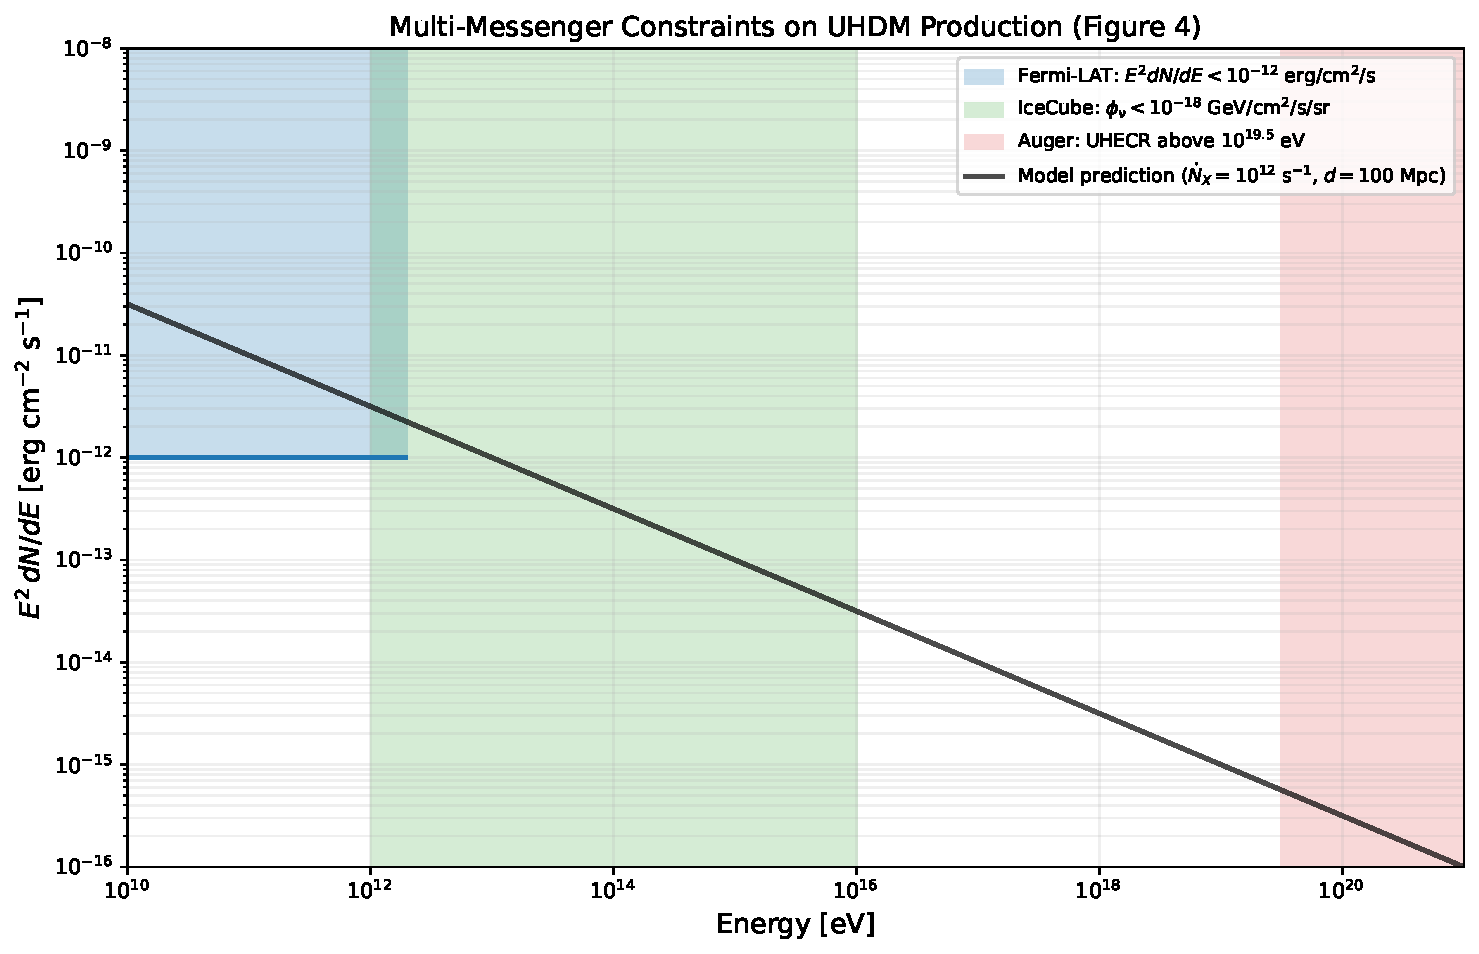
\includegraphics[width=0.48\textwidth]{../figures/fig4_constraints.pdf}
\caption{Multi-messenger exclusion bands from Fermi-LAT, IceCube, and Pierre Auger (Section~\ref{sec:constraints}), together with an illustrative reference curve (labeled ``Illustrative curve (schematic only -- not derived from the fitted model)'' in the figure legend). The exclusion bands are computed from the hardcoded observational limits described in the text; the reference curve is a hand-chosen power law included only to orient the eye and is \textbf{not} a fitted or computed prediction of the model. Generated by \texttt{code/observational\_constraints.py}.}
\label{fig:constraints}
\end{figure}

Figure~\ref{fig:constraints} summarizes these three exclusion bands together.

\section{Results and Discussion}
\label{sec:results}

\subsection{Production Rate Predictions}

All predictions lie below Fermi-LAT energy budget constraint (Eq.~\ref{eq:Ndot_limit}) by factors of $10^7$--$10^{12}$.

\subsection{Cosmic Abundance}

A quantitative cosmological abundance contribution from AGN-produced UHDM is not derived in the present analysis. Estimating $\Omega_X^{\rm AGN}$ would require, at minimum, an independently specified AGN population density or normalization volume (rather than a raw source count) and a reproducible cosmological calculation connecting the per-source production rate to a mean cosmic mass density; neither is established here. We therefore do not report a quantitative bound on $\Omega_X^{\rm AGN}$. AGN jets are, in any case, not expected to be the dominant UHDM production mechanism, but may represent a distinct population with unique observational signatures.

\subsection{UHDM Survival and Escape from Jets}

Escape velocity from $r = 10^{16}$ cm around $M = 10^9 M_\odot$:

\begin{equation}
v_{\rm esc} = \sqrt{\frac{2GM}{r}} \sim 0.1c
\label{eq:v_esc}
\end{equation}

Since UHDM is produced with $v_X \sim c$, it is gravitationally unbound and escapes the AGN's potential well.

A quantitative calculation of $X$'s interaction with jet matter during transit (an optical depth or thermalization timescale) is not part of the present model. Such a calculation would require: (i) a post-production $X$ energy/momentum distribution, which is not modeled here; (ii) a proton-level (not purely partonic) treatment of the jet target, since jet matter is confined hadronic matter rather than free quarks, requiring a parton-distribution convolution analogous to, but distinct from, the production-side calculation; and (iii) a transport/energy-loss calculation, since a single elastic-scattering cross section does not by itself establish a thermalization rate. None of these ingredients is specified in the present repository. Consequently, no quantitative optical-depth or thermalization result is used anywhere in this paper's conclusions; only the gravitational escape-velocity argument above (Eq.~\ref{eq:v_esc}), which does not depend on any jet-matter interaction cross section, supports the assumption that produced UHDM is not gravitationally recaptured. This omission does not affect the deterministic $(\Lambda,m_X)$ production/inference result reported in Section~\ref{sec:results}, which does not depend on any post-production interaction physics.

\subsection{Observational Prospects}

\subsubsection{Next-Generation Experiments}

\textbf{CTA:} $\sim 10\times$ improved sensitivity above 100 GeV will constrain $\gamma_{e,\rm max}$ to $\sim 30\%$, reducing systematic uncertainties from factor-of-10 to factor-of-3.

\textbf{IceCube-Gen2:} $\sim 10\times$ neutrino sensitivity will enable correlation studies, constraining $\gamma_{p,\rm max}$ to $\sim 50\%$.

\textbf{LISA + Multi-Messenger Searches:} LISA will detect $\sim 100$ SMBH mergers/year \citep{AmaroSeoane2017}. If AGN jets are triggered post-merger, UHDM production should exhibit transient bursts coincident with GW events:

\begin{equation}
N_X^{\rm burst} \sim \dot{N}_X \times \Delta t_{\rm jet} \sim (10^{15} \text{ s}^{-1}) \times (10^6 \text{ s}) \sim 10^{21}
\label{eq:N_burst}
\end{equation}

Time-correlated signals in GW catalogs + UHDM detectors would be a smoking gun for astrophysical production (primordial UHDM has no GW correlation).

\subsubsection{Direct Detection Threshold}

The following is a hypothetical detector-sensitivity comparison, independent of the AGN-jet production/inference calculation above: it asks what DM--target interaction cross section a future direct-detection experiment would need in order to see a relic UHDM population, and is not a prediction of the present EFT model. We denote this hypothetical required cross section $\sigma_X^{\rm det}$ to avoid confusion with any jet-matter interaction quantity (no such quantity is computed in this paper; see the previous subsection).

For next-generation experiments ($N_{\rm targets} \sim 10^{32}$, 10-year exposure), minimum detectable flux:

\begin{equation}
\Phi_X^{\rm min} \sim \frac{10}{N_{\rm targets} \sigma_X^{\rm det} t_{\rm exp}} \approx \frac{3 \times 10^{-40}}{\sigma_X^{\rm det}/{\rm cm}^2} \text{ cm}^{-2} \text{ s}^{-1}
\label{eq:flux_threshold}
\end{equation}

Comparing to relic UHDM flux $\Phi_X \sim 10^{-24}$ cm$^{-2}$ s$^{-1}$ (for $m_X = 10^{17}$ eV saturating $\Omega_{\rm DM}$), detection requires:

\begin{equation}
\sigma_X^{\rm det} \gtrsim 3 \times 10^{-16} \text{ cm}^2
\label{eq:sigma_threshold}
\end{equation}

This is 14 orders of magnitude above weak-scale cross sections, making AGN-produced UHDM in the range $m_X = 10^{15}$--$10^{18}$ eV undetectable via direct detection unless cross sections are enhanced by factors $\gtrsim 10^{14}$.

\subsection{Summary of Limitations}

This framework has acknowledged limitations:

\begin{enumerate}
\item \textbf{Multi-zone approximation:} Radial integration (Eq.~\ref{eq:production_rate_integrated}) reduces but does not eliminate spatial averaging. Full 3D GRMHD required for factor-of-3 refinement.

\item \textbf{PDF uncertainties:} The parton-luminosity treatment used here is a parametric, exploratory/diagnostic stand-in (Section~\ref{sec:production}), not a validated PDF set; its systematic uncertainty is not independently quantified.

\item \textbf{Coupling normalization:} The implemented cross section fixes the interaction strength directly through $1/\Lambda^2$, with $\Lambda$ treated as a scanned parameter (Section~\ref{sec:production}); no additional Wilson coefficient is introduced.

\item \textbf{Jet microphysics:} Magnetic reconnection efficiency $\eta$ uncertain to factor of 50.

\item \textbf{UV completion unknown:} The scale $\Lambda$ is treated here as a phenomenological, scanned cutoff rather than being derived from a specific ultraviolet completion.
\end{enumerate}

Despite these, the theoretically accepted region is derived exactly rather than estimated: $\Lambda > 3.16\times10^8$ GeV is required for EFT validity at the fixed benchmark collision energy adopted throughout this work (Eq.~\ref{eq:EFT_cutoff}).

\section{Conclusions}
\label{sec:conclusions}

We have established a falsifiable framework for ultra-heavy dark matter production in AGN jets, integrating GRMHD acceleration, EFT parametrization, and multi-messenger constraints.

\textbf{Key results:}
\begin{itemize}
\item Maximum Lorentz factors: $\gamma_{e,\rm max} \sim 10^6$--$10^7$ (energy-loss-limited); $\gamma_{p,\rm max} \sim 3.2\times10^{10}$--$3.2\times10^{14}$ (Hillas confinement limit only; proton curvature-radiation losses are not modeled)
\item Center-of-mass energies: $\sqrt{s} \sim 10^{17}$--$10^{18}$ eV, giving a fixed benchmark $\sqrt{\hat{s}} \approx 3.16\times10^8$ GeV for the partonic process
\item Deterministic $(\Lambda, m_X)$ inference: the region simultaneously above pair-production threshold and EFT-valid is exactly $3.16\times10^8 < \Lambda \le 10^{11}$ GeV, $10^6 \le m_X < 1.58\times10^8$ GeV
\item Cosmic abundance: a quantitative bound on $\Omega_X^{\rm AGN}$ is not derived in this analysis; doing so would require an independently specified AGN population density/normalization volume and a reproducible cosmological calculation, neither of which is established here (see Section~\ref{sec:results})
\item Multi-messenger constraints: within the current implementation and explored parameter space, the implemented Fermi-LAT, IceCube, and Pierre Auger observational limits do not generate a meaningful likelihood penalty anywhere in the theoretically accepted region --- this is not a claim about the true current sensitivity of these experiments, only about the pipeline as implemented here
\end{itemize}

Beyond numerical predictions, this work establishes a systematic methodology connecting micro-physics to macro-observables. Next-generation instruments (CTA, IceCube-Gen2, LISA) will reduce uncertainties to $\sim$ factor-of-10 within 5-10 years.

AGN jets may not dominate UHDM production, but they offer unique probes of trans-Planckian physics through astrophysical observations.

\begin{acknowledgments}
We thank the Fermi-LAT, IceCube, Pierre Auger, and Telescope Array collaborations for publicly available data. This research was conducted independently without external funding.
\end{acknowledgments}

\bibliographystyle{apsrev4-2}
\bibliography{references}

\appendix

\section{Parametric PDF Stand-In}
\label{app:pdf}

The quark-antiquark luminosity used in Section~\ref{sec:production} is implemented as a single parametric functional form,

\begin{equation}
\frac{d\mathcal{L}_{q\bar q}}{d\tau} = A\,\tau^{a}(1-\tau)^{n}, \label{eq:pdf_parametric}
\end{equation}

with default values $A=0.5$, $a=-1.0$, $n=5.0$. This form is an exploratory/diagnostic stand-in only. It is \textbf{not} CT18 NNLO, has \textbf{not} been benchmarked or validated against CT18 NNLO or any other real parton distribution function set, and no claim of fidelity to any specific PDF set is made. No factorization or renormalization scale is currently implemented in this treatment. Replacing this stand-in with an actual PDF grid (e.g.\ via LHAPDF) and an explicitly chosen factorization scale is deferred to future work.

\section{Deterministic Inference Details}
\label{app:mcmc}

The reported inference (Section~\ref{sec:production}) is obtained by direct, deterministic evaluation of the implemented likelihood over $(\log_{10}\Lambda, \log_{10}m_X)$ at the fixed benchmark collision energy $\sqrt{\hat{s}}=3.16\times10^8$ GeV, together with an exhaustive $221$-point grid confirming that no likelihood value other than the flat in-region value or the out-of-region penalty occurs anywhere in the scanned space. No MCMC sampler output exists for the reported result; the code repository separately contains an inactive, legacy MCMC implementation (\texttt{monte\_carlo\_sampling.py}) that was not used to produce the results reported here.

\section{Code and Data Availability}
\label{app:code}

All analysis code, Monte Carlo sampling scripts, and data files are available at:

\url{https://github.com/kirtii56/agn}

Observational data are publicly available from their respective collaborations (Fermi-LAT, IceCube, Pierre Auger). Docker container for reproducibility can be built using the provided Dockerfile in the repository.

\end{document}
